% Generated from locale/tr/content/history/set-theory/limits.tex; do not hand-edit.

	
\olfileid[tr]{his}{set}{limits}	

\olsection{Limitlerin Kesin Tanımı}
	
Günümüzde yukarıdaki problemin standart çözümü sonsuz küçükleri ortadan
kaldırmaktır. Bunun nasıl yapıldığını görelim.

$\beta$ küçüldükçe eğime ilişkin daha iyi yaklaşımlar elde ettiğimizi gördük.
Gerçekten de $\beta$, $0$'a istediğimiz kadar yaklaştığında $f'(c)$'nin değeri
istediğimiz eğime ``sınırsızca yaklaşır''. Öyleyse $\beta = 0$ \emph{iken}
ne olduğunu ele almak yerine, yalnızca $f'(c)$'nin, $\beta$ $0$'a yaklaşırken
gösterdiği \emph{eğilimi} ele almamız gerekir.

Bu biçimde ortaya konduğunda genel güçlük, şu biçimdeki iddiaları
anlamlandırmaktır:
\begin{center}
$x$, $c$'ye yaklaşırken $g(x)$, $\ell$'ye sınırsızca yaklaşır.
\end{center}
Bunu daha kısa olarak şöyle yazabiliriz:
\[
\lim_{x \rightarrow c}g(x) = \ell.
\]
Weierstrass, 19. yüzyılda Cauchy'nin daha önceki çalışmalarına dayanarak bu
ifadenin bütünüyle kesin bir tanımını verdi. Fikir gerçekten de $g(x)$'i
$\ell$'ye istediğimiz kadar yaklaştırabilmemizdir; bunun için $x$'i $c$'ye
uygun ölçüde yaklaştırırız. Daha kesin söylersek $\lim_{x \rightarrow c} g(x) =
\ell$ ifadesinin şu anlama gelmesini kararlaştırırız:
\[
(\forall\epsilon > 0)(\exists \delta > 0)\forall x \left(0 < |x - c| < \delta \lif |g(x) - \ell| < \epsilon \right).
\]
Buradaki dikey çizgiler mutlak değeri gösterir. Başka bir deyişle $|x| = x$
eşitliği $x \geq 0$ iken, $|x| =-x$ eşitliği de $x < 0$ iken geçerlidir;
\emph{bu} fonksiyonu şöyle çizebilirsiniz:
\begin{center}
	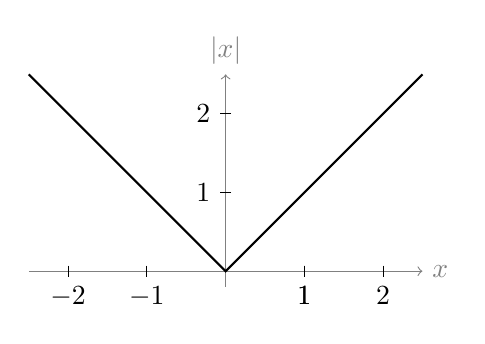
\begin{tikzpicture}[scale=1]
	\draw[->, gray] (-2.5,0) -- (2.5,0) node[right] {$x$};
	\draw[->, gray] (0,-.2) -- (0,2.5) node[above] {$|x|$};
	
	\foreach \x/\xtext in {-2/-2, -1,1, 1/1, 2/2}
	\draw[shift={(\x,0)}] (0pt,2pt) -- (0pt,-2pt) node[below] {{$\xtext$}};
	
	\foreach \y/\ytext in {1/1, 2/2}
	\draw[shift={(0,\y)}] (2pt,0pt) -- (-2pt,0pt) node[left] {{$\ytext$}};
	
	\draw[thick] (-2.5, 2.5)--(0,0)--(2.5, 2.5);
	\end{tikzpicture}
\end{center}
Öyleyse tanım kabaca şunu söyler: ``Hatanızı'' $\epsilon$'dan küçük (yani
$|g(x) - \ell| < \epsilon$) kılabilirsiniz; bunun için $\delta$'dan fazla
uzakta olmayan argümanları $c$ çevresinden seçersiniz (yani
$0 < |x - c| < \delta$).

Limit kavramını tanımladıktan sonra, $f$'nin $c$'deki eğiminin şu formülle
verildiğini kararlaştırarak sonsuz küçüklerden tümüyle kaçınabiliriz:
\[
	{f}'(c) = \lim_{x \rightarrow 0}\left(\frac{f(c +x) - f(c)}{x}\right) \text{; limitin var olduğu durumda.}
\]
Ancak tanımımızın neden ``limitin var olduğu durumda'' kaydına ihtiyaç
duyduğunu anlamak önemlidir. Basit bir örnek olarak grafiğini az önce
gördüğümüz $f(x) = |x|$ fonksiyonunu ele alın. $f'(0)$'ın iyi tanımlı
olmadığı açıktır: $0$'a ``sağdan'' yaklaşırsak eğim her zaman $1$'dir;
$0$'a ``soldan'' yaklaşırsak eğim her zaman $-1$'dir; dolayısıyla limit
tanımsızdır. Buna göre bir $f$ fonksiyonunun, ancak ve ancak böyle bir limit
varsa $x$'te \emph{türevlenebilir} olduğunu ekleyebiliriz.

\emph{Limit} kavramını kullanarak türev almayı nasıl ele alacağımızı gördük.
Aynı kavramı \emph{sürekli} fonksiyon fikrini tanımlamak için de
kullanabiliriz. (Bolzano aslında bunu 1817'ye gelindiğinde fark etmişti.)
Sürekliliğin Cauchy--Weierstrass tarafından ele alınışı şöyledir. Kabaca: Bir
$f$ fonksiyonu, çıktısı için belirli bir kesinlik düzeyi istediğinizde bunu
girdisi için belirli bir kesinlik düzeyinde ısrar ederek güvence altına
alabiliyorsanız (bir noktada) süreklidir. Daha kesin söylersek $f$, $c$'de şu
koşulla süreklidir: $x$ sıfıra yaklaşırken $f(c + x)$ ile $f(c)$ arasındaki
farkın kendisi $0$'a yaklaşır. Başka bir deyişle $f$, $c$'de ancak ve ancak
$f(c) = \lim_{x \rightarrow c} f(x)$ ise \emph{süreklidir}.

Daha ileri gitmek, konumuz küme teorisiyken bizi gerçel analize sürükler.
Öyleyse burada durup çıkarılacak dersi belirtmeliyiz. Matematikçiler 19.
yüzyılda, kesin biçimde tanımlanmış bir \emph{limit} kavramına başvurarak
sonsuz küçükler olmadan çalışmayı öğrendiler.

